% Today we're going to learn/remember how to use Venn Diagrams in latex.

% Open document format
\documentclass{article}

% Now call the package we use to make the diagrams
\usepackage{tikz}

\title{Venn Diagrams in Latex}
\author{Sofia Silva}

% Open document environment
\begin{document}

\maketitle

The Venn diagram, or set diagram, was invented by John Venn in 1880 in order to visualize the relationships between sets. 

\section{Disjointed Circles}
% Open the package environment
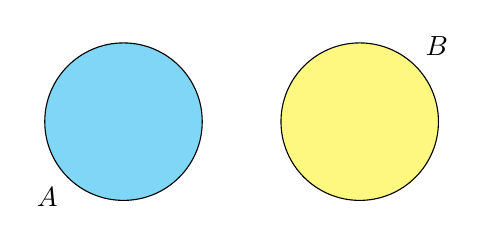
\begin{tikzpicture}

% This was the model provided which works

% Circle with lable at 225 deg
\node[draw,
    circle,
    minimum size =2cm,
    fill=cyan!50,
    label={225:$A$}] (circle1) at (0,0){};
    
% Circle with label at 45 deg.
\node[draw,
    circle,
    minimum size =2cm,
    fill=yellow!50,
    label={45:$B$}] (circle2) at (3,0){};

% Close the package environment
\end{tikzpicture}



\section{Intersected circles}
% Open the package environment
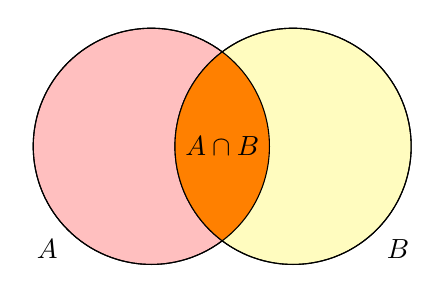
\begin{tikzpicture}

% Circle 1
\node[draw,
    circle,
    minimum size =3cm,
    fill=red!25,
    label={225:$A$}] (A) at (0,0){}; %{degrees:label} 
    
% Circle 2
\node[draw,
    circle,
    minimum size =3cm,
    fill=yellow!25,
    label={315:$B$}] (B) at (1.8,0){};
    
% Intersection fill
\begin{scope}
	\clip (0,0) circle(1.5cm);
	\clip (1.8,0) circle(1.5cm);
	\fill[orange] (0,0) circle (1.5cm);
\end{scope}
    
% Outline Circles because overlap will hide circles
\draw[black] (0,0) circle (1.5cm);
\draw[black] (1.8,0) circle (1.5cm);
    
% Set intersection label
\node at (0.9,0) {$A\cap B$};

% Close the package environment
\end{tikzpicture}

\section{Complimented Circles Example}
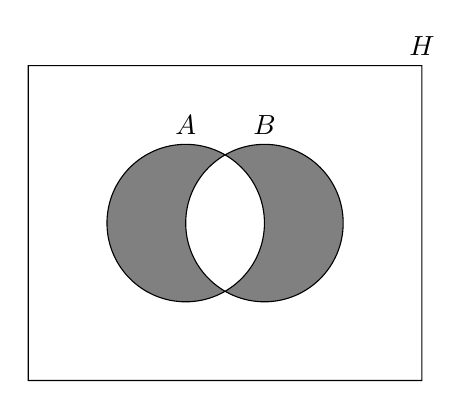
\begin{tikzpicture}[fill=gray]
% left hand
\scope
\clip (-2,-2) rectangle (2,2)
      (1,0) circle (1);
\fill (0,0) circle (1);
\endscope
% right hand
\scope
\clip (-2,-2) rectangle (2,2)
      (0,0) circle (1);
\fill (1,0) circle (1);
\endscope
% outline
\draw (0,0) circle (1) (0,1)  node [text=black,above] {$A$}
      (1,0) circle (1) (1,1)  node [text=black,above] {$B$}
      (-2,-2) rectangle (3,2) node [text=black,above] {$H$};
\end{tikzpicture}

\section{My Attempt}
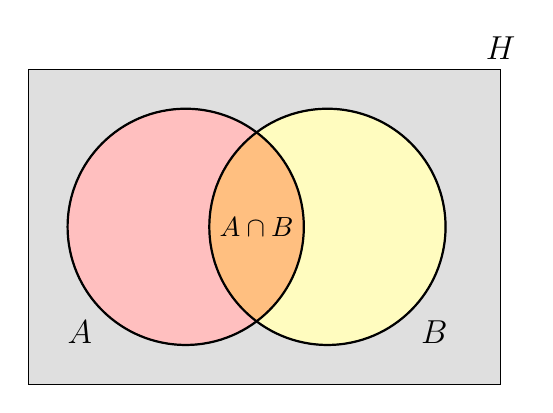
\begin{tikzpicture}

\filldraw[fill=gray!25] (-2,-2) rectangle (4,2);

\node[draw,
    circle,
    minimum size =3cm,
    fill=red!25,
    label={[black,font=\large]225:$A$}] (circle1) at (0,0){}; %{degrees:label} 
    
% Circle 2
\node[draw,
    circle,
    minimum size =3cm,
    fill=yellow!25,
    label={[black,font=\large]315:$B$}] (B) at (1.8,0){};
    
% Intersection fill
\begin{scope}
	\clip (0,0) circle(1.5);
	\clip (1.8,0) circle(1.5);
	\fill[orange!50] (0,0) circle (1.5);
\end{scope}
    
% Outline Circles because overlap will hide circles
\draw[black,thick] (0,0) circle (1.5);
\draw[black,thick] (1.8,0) circle (1.5);
\draw[black] (-2,-2) rectangle (4,2) node [text=black,above,font=\large] {$H$};
    
% Set intersection label
\node[text=black,thick] at (0.9,0) {$A\cap B$};

\end{tikzpicture}

% Close document environment
\end{document}